% !TeX program = lualatex
\documentclass{beamer}
\usetheme[progressbar=frametitle]{metropolis}
\usepackage{appendixnumberbeamer}

\usepackage{booktabs}
\usepackage[scale=2]{ccicons}

\usepackage{pgfplots}
\usepgfplotslibrary{dateplot}

\usepackage{xspace}
\newcommand{\themename}{\textbf{\textsc{metropolis}}\xspace}
\title{Attention based models in End-to-End ASR}
\subtitle{Exploration of Attention in ESPNET toolkit}
\date{\today}
\author{Shreekantha Nadig}
\institute{International Institute of Information Technology - Bangalore}
%\titlegraphic{\hfill\includegraphics[height=1.5cm]{logo.pdf}}

\usepackage{tikz}
\usetikzlibrary{shapes,shadows,arrows, patterns}


\tikzstyle{line} = [draw, -latex']
\tikzstyle{round} = [draw, circle, fill=black!30, minimum size=4em, node distance=4em, font=\fontsize{30}{10}\selectfont]
\tikzstyle{mlp_enc} = [rectangle, draw, fill=red!50, text width=2cm, minimum height=5em, text centered, node distance=10em, font=\fontsize{20}{10}\selectfont]
\tikzstyle{mlp_att} = [rectangle, draw, fill=green!50, text width=2cm, minimum height=5em, text centered, node distance=10em, font=\fontsize{20}{10}\selectfont]
\tikzstyle{mlp_dec} = [rectangle, draw, fill=blue!50, text width=2cm, minimum height=5em, text centered, node distance=10em, font=\fontsize{20}{10}\selectfont]
\tikzstyle{enc_h} = [rectangle, draw,  pattern=horizontal lines, pattern color=red!60, text width=1cm, minimum height=10em, minimum width=3em, text centered, node distance=10em, font=\fontsize{25}{10}\selectfont]
\tikzstyle{atts} = [rectangle, draw,  pattern=horizontal lines, pattern color=green!70, text width=1cm, minimum height=10em, minimum width=3em, text centered, node distance=10em, font=\fontsize{20}{10}\selectfont]
\tikzstyle{dec_z} = [rectangle, draw,  pattern=horizontal lines, pattern color=blue!60, text width=1cm, minimum height=10em, minimum width=3em, text centered, node distance=10em, font=\fontsize{20}{10}\selectfont]
\tikzstyle{cnn} = [rectangle, draw,  pattern=crosshatch, pattern color=red!50!blue!50, text width=2cm, minimum height=5em, text centered, node distance=10em, font=\fontsize{20}{10}\selectfont]
\tikzstyle{box} = [rectangle, draw,  fill=blue!20, text width=3cm, minimum height=5em, minimum width=3em, text centered, node distance=10em, font=\fontsize{20}{10}\selectfont]

\begin{document}

\maketitle
\begin{frame}{Table of contents}
\setbeamertemplate{section in toc}[sections numbered]
\tableofcontents[hideallsubsections]
\end{frame}

\section{Introduction}
\begin{frame}[fragile]{BLSTM}
	\begin{center}
	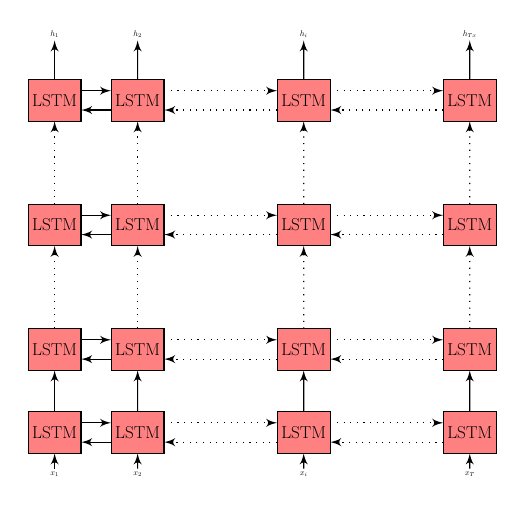
\begin{tikzpicture}[scale=0.3, every node/.style={transform shape}]
			\onslide<1->\node[mlp_enc](LSTM_1_1){LSTM};
			\node[mlp_enc, right of=LSTM_1_1](LSTM_1_2) {LSTM};
			\path [line] (LSTM_1_1.20) to (LSTM_1_1.20-|LSTM_1_2.west);
			\path [line] (LSTM_1_2.200) to (LSTM_1_2.-20-|LSTM_1_1.east);     
			
			\node[mlp_enc, right of=LSTM_1_2, node distance = 20em](LSTM_1_i) {LSTM};
			\path [line, dotted] (LSTM_1_2.20) to (LSTM_1_2.20-|LSTM_1_i.west);
			\path [line, dotted] (LSTM_1_i.200) to (LSTM_1_i.200-|LSTM_1_2.east);
			
			\node[mlp_enc, right of=LSTM_1_i, node distance = 20em](LSTM_1_Tx) {LSTM};
			\path [line, dotted] (LSTM_1_i.20) to (LSTM_1_i.20-|LSTM_1_Tx.west);
			\path [line, dotted] (LSTM_1_Tx.200) to (LSTM_1_Tx.200-|LSTM_1_i.east);
			
			\node [below of=LSTM_1_1, node distance = 5em] (x1) {$x_{1}$};
			\node [below of=LSTM_1_2, node distance = 5em] (x2) {$x_{2}$};
			\node [below of=LSTM_1_i, node distance = 5em] (xi) {$x_{i}$};
			\node [below of=LSTM_1_Tx, node distance = 5em] (xTx) {$x_{T}$};
			
			\path [line] (x1) to (LSTM_1_1);
			\path [line] (x2) to (LSTM_1_2);
			\path [line] (xi) to (LSTM_1_i);
			\path [line] (xTx) to (LSTM_1_Tx);
			
			\onslide<2->\node[mlp_enc, above of = LSTM_1_1](LSTM_2_1){LSTM};
			\node[mlp_enc, right of=LSTM_2_1](LSTM_2_2) {LSTM};
			\path [line] (LSTM_2_1.20) to (LSTM_2_1.20-|LSTM_2_2.west);
			\path [line] (LSTM_2_2.200) to (LSTM_2_2.-20-|LSTM_2_1.east);     
			
			\node[mlp_enc, right of=LSTM_2_2, node distance = 20em](LSTM_2_i) {LSTM};
			\path [line, dotted] (LSTM_2_2.20) to (LSTM_2_2.20-|LSTM_2_i.west);
			\path [line, dotted] (LSTM_2_i.200) to (LSTM_2_i.200-|LSTM_2_2.east);
			
			\node[mlp_enc, right of=LSTM_2_i, node distance = 20em](LSTM_2_Tx) {LSTM};
			\path [line, dotted] (LSTM_2_i.20) to (LSTM_2_i.20-|LSTM_2_Tx.west);
			\path [line, dotted] (LSTM_2_Tx.200) to (LSTM_2_Tx.200-|LSTM_2_i.east);
			
			\path [line] (LSTM_1_1) to (LSTM_2_1);
			\path [line] (LSTM_1_2) to (LSTM_2_2);
			\path [line] (LSTM_1_i) to (LSTM_2_i);
			\path [line] (LSTM_1_Tx) to (LSTM_2_Tx);
			
			\node[mlp_enc, above of = LSTM_2_1, node distance = 15em](LSTM_i_1){LSTM};
			\node[mlp_enc, right of=LSTM_i_1](LSTM_i_2) {LSTM};
			\path [line] (LSTM_i_1.20) to (LSTM_i_1.20-|LSTM_i_2.west);
			\path [line] (LSTM_i_2.200) to (LSTM_i_2.-20-|LSTM_i_1.east);     
			
			\node[mlp_enc, right of=LSTM_i_2, node distance = 20em](LSTM_i_i) {LSTM};
			\path [line, dotted] (LSTM_i_2.20) to (LSTM_i_2.20-|LSTM_i_i.west);
			\path [line, dotted] (LSTM_i_i.200) to (LSTM_i_i.200-|LSTM_i_2.east);
			
			\node[mlp_enc, right of=LSTM_i_i, node distance = 20em](LSTM_i_Tx) {LSTM};
			\path [line, dotted] (LSTM_i_i.20) to (LSTM_i_i.20-|LSTM_i_Tx.west);
			\path [line, dotted] (LSTM_i_Tx.200) to (LSTM_i_Tx.200-|LSTM_i_i.east);
			
			\path [line, dotted] (LSTM_2_1) to (LSTM_i_1);
			\path [line, dotted] (LSTM_2_2) to (LSTM_i_2);
			\path [line, dotted] (LSTM_2_i) to (LSTM_i_i);
			\path [line, dotted] (LSTM_2_Tx) to (LSTM_i_Tx);
			
			
			\onslide<4->\node[mlp_enc, above of = LSTM_i_1, node distance = 15em](LSTM_N_1){LSTM};
			\node[mlp_enc, right of=LSTM_N_1](LSTM_N_2) {LSTM};
			\path [line] (LSTM_N_1.20) to (LSTM_N_1.20-|LSTM_N_2.west);
			\path [line] (LSTM_N_2.200) to (LSTM_N_2.-20-|LSTM_N_1.east);     
			
			\node[mlp_enc, right of=LSTM_N_2, node distance = 20em](LSTM_N_i) {LSTM};
			\path [line, dotted] (LSTM_N_2.20) to (LSTM_N_2.20-|LSTM_N_i.west);
			\path [line, dotted] (LSTM_N_i.200) to (LSTM_N_i.200-|LSTM_N_2.east);
			
			\node[mlp_enc, right of=LSTM_N_i, node distance = 20em](LSTM_N_Tx) {LSTM};
			\path [line, dotted] (LSTM_N_i.20) to (LSTM_N_i.20-|LSTM_N_Tx.west);
			\path [line, dotted] (LSTM_N_Tx.200) to (LSTM_N_Tx.200-|LSTM_N_i.east);
			
			\path [line, dotted] (LSTM_i_1) to (LSTM_N_1);
			\path [line, dotted] (LSTM_i_2) to (LSTM_N_2);
			\path [line, dotted] (LSTM_i_i) to (LSTM_N_i);
			\path [line, dotted] (LSTM_i_Tx) to (LSTM_N_Tx);

			\onslide<5->\node [above of = LSTM_N_1, node distance = 8em] (h1) {$h_{1}$};
			\node [above of = LSTM_N_2, node distance = 8em] (h2) {$h_{2}$};
			\node [above of = LSTM_N_i, node distance = 8em] (hi) {$h_{i}$};
			\node [above of = LSTM_N_Tx, node distance = 8em] (hTx) {$h_{Tx}$};
			
			\path [line] (LSTM_N_1) to (h1);
			\path [line] (LSTM_N_2) to (h2);
			\path [line] (LSTM_N_i) to (hi);
			\path [line] (LSTM_N_Tx) to (hTx);
	\end{tikzpicture}
	\end{center}
	\end{frame}
	
	\begin{frame}[fragile]{Introduction to Attention}
		\begin{center}
			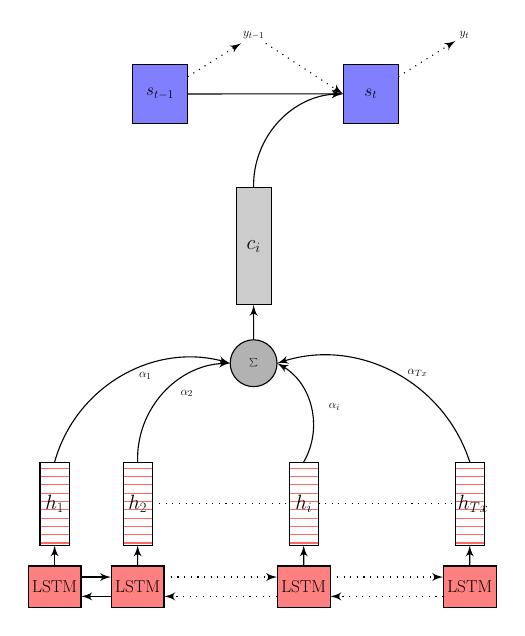
\begin{tikzpicture}[scale=0.3, every node/.style={transform shape}]
				\node[mlp_enc, node distance = 15em](LSTM_N_1){LSTM};
				\node[mlp_enc, right of=LSTM_N_1](LSTM_N_2) {LSTM};
				\path [line] (LSTM_N_1.20) to (LSTM_N_1.20-|LSTM_N_2.west);
				\path [line] (LSTM_N_2.200) to (LSTM_N_2.-20-|LSTM_N_1.east);     
				
				\node[mlp_enc, right of=LSTM_N_2, node distance = 20em](LSTM_N_i) {LSTM};
				\path [line, dotted] (LSTM_N_2.20) to (LSTM_N_2.20-|LSTM_N_i.west);
				\path [line, dotted] (LSTM_N_i.200) to (LSTM_N_i.200-|LSTM_N_2.east);
				
				\node[mlp_enc, right of=LSTM_N_i, node distance = 20em](LSTM_N_Tx) {LSTM};
				\path [line, dotted] (LSTM_N_i.20) to (LSTM_N_i.20-|LSTM_N_Tx.west);
				\path [line, dotted] (LSTM_N_Tx.200) to (LSTM_N_Tx.200-|LSTM_N_i.east);
				
				
				\node [enc_h, above of = LSTM_N_1] (h1) {$h_{1}$};
				\node [enc_h,above of = LSTM_N_2] (h2) {$h_{2}$};
				\node [enc_h,above of = LSTM_N_i] (hi) {$h_{i}$};
				\node [enc_h,above of = LSTM_N_Tx] (hTx) {$h_{Tx}$};

				\draw [dotted] (h2.east) to (hi.west);
				\draw [dotted] (hi.east) to (hTx.west);

				\path [line] (LSTM_N_1) to (h1);
				\path [line] (LSTM_N_2) to (h2);
				\path [line] (LSTM_N_i) to (hi);
				\path [line] (LSTM_N_Tx) to (hTx);
				
				
				\pause{}
				\fontsize{15}{12}
				\node [round, above of = h1, node distance = 12em, xshift=17em] (sum1) {$\sum$};
				
				\pause{}
				\path [line] (h1.north) to [bend left=45] node [xshift=2em] {$\alpha_{1}$} (sum1.west);
				\pause{}
				\path [line] (h2.north) to [bend left=45] node [xshift=2em] {$\alpha_{2}$} (sum1.west);
				\pause{}
				\path [line] (hi.north) to [bend right=45] node [xshift=2em] {$\alpha_{i}$} (sum1.east);
				\pause{}
				\path [line] (hTx.north) to [bend right=45] node [xshift=2em] {$\alpha_{Tx}$} (sum1.east);

				\pause{}
				\node [enc_h, above of = sum1, fill=black!20] (ci) {$c_{i}$};
				
				\path [line] (sum1) to (ci.south);
				
				\pause{}
				\node [mlp_dec, above of = ci, xshift = -8em, yshift = 3em] (decoder_tm1) {$s_{t-1}$};
				\node [above of = decoder_tm1, node distance = 5em, xshift = 8em] (ytm1) {$y_{t-1}$};
				\path [line, dotted] (decoder_tm1) to (ytm1);
				\pause{}
				\pause{}
				\node [mlp_dec, right of = decoder_tm1, xshift = 8em] (decoder_t) {$s_{t}$};
				\path [line] (decoder_tm1.east) to (decoder_t.west);
				\path [line] (ci.north) to [bend left=45] (decoder_t.west);
				\path [line, dotted] (ytm1) to (decoder_t.west);
				\pause{}
				\node [above of = decoder_t, node distance = 5em, xshift = 8em] (yt) {$y_{t}$};
				\path [line, dotted] (decoder_t) to (yt);
			\end{tikzpicture}
		\end{center}
	\end{frame}

	\begin{frame}[fragile]{No Attention [Equal Attention?]}
	\begin{center}
	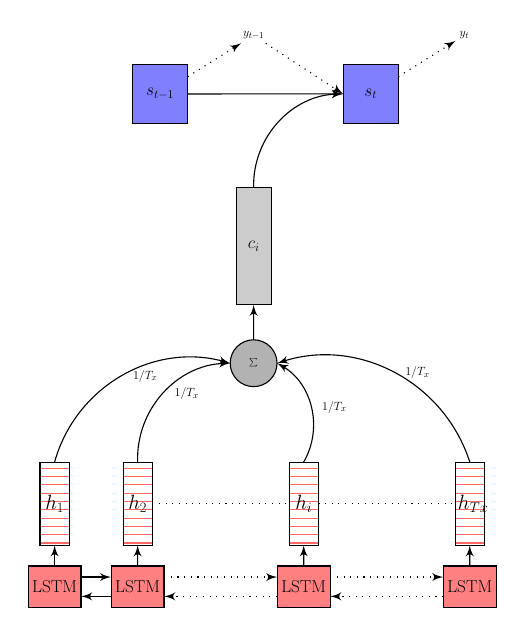
\begin{tikzpicture}[scale=0.3, every node/.style={transform shape}]
		\node[mlp_enc, node distance = 15em](LSTM_N_1){LSTM};
		\node[mlp_enc, right of=LSTM_N_1](LSTM_N_2) {LSTM};
		\path [line] (LSTM_N_1.20) to (LSTM_N_1.20-|LSTM_N_2.west);
		\path [line] (LSTM_N_2.200) to (LSTM_N_2.-20-|LSTM_N_1.east);     
		
		\node[mlp_enc, right of=LSTM_N_2, node distance = 20em](LSTM_N_i) {LSTM};
		\path [line, dotted] (LSTM_N_2.20) to (LSTM_N_2.20-|LSTM_N_i.west);
		\path [line, dotted] (LSTM_N_i.200) to (LSTM_N_i.200-|LSTM_N_2.east);
		
		\node[mlp_enc, right of=LSTM_N_i, node distance = 20em](LSTM_N_Tx) {LSTM};
		\path [line, dotted] (LSTM_N_i.20) to (LSTM_N_i.20-|LSTM_N_Tx.west);
		\path [line, dotted] (LSTM_N_Tx.200) to (LSTM_N_Tx.200-|LSTM_N_i.east);
		
		
		\node [enc_h, above of = LSTM_N_1] (h1) {$h_{1}$};
		\node [enc_h,above of = LSTM_N_2] (h2) {$h_{2}$};
		\node [enc_h,above of = LSTM_N_i] (hi) {$h_{i}$};
		\node [enc_h,above of = LSTM_N_Tx] (hTx) {$h_{Tx}$};
		
		\path [line] (LSTM_N_1) to (h1);
		\path [line] (LSTM_N_2) to (h2);
		\path [line] (LSTM_N_i) to (hi);
		\path [line] (LSTM_N_Tx) to (hTx);

		\draw [dotted] (h2.east) to (hi.west);
		\draw [dotted] (hi.east) to (hTx.west);
		
		
		\fontsize{15}{12}
		\node [round, above of = h1, node distance = 12em, xshift=17em] (sum1) {$\sum$};
		
		
		\path [line] (h1.north) to [bend left=45] node [xshift=2em] {$1/T_x$} (sum1.west);
		
		\path [line] (h2.north) to [bend left=45] node [xshift=2em] {$1/T_x$} (sum1.west);
		
		\path [line] (hi.north) to [bend right=45] node [xshift=2em] {$1/T_x$} (sum1.east);
		
		\path [line] (hTx.north) to [bend right=45] node [xshift=2em] {$1/T_x$} (sum1.east);
		
		
		\node [atts, above of = sum1, fill=black!20] (ci) {$c_{i}$};
		
		\path [line] (sum1) to (ci.south);
		
		
		\node [mlp_dec, above of = ci, xshift = -8em, yshift = 3em] (decoder_tm1) {$s_{t-1}$};
		\node [above of = decoder_tm1, node distance = 5em, xshift = 8em] (ytm1) {$y_{t-1}$};
		\path [line, dotted] (decoder_tm1) to (ytm1);
		
		
		\node [mlp_dec, right of = decoder_tm1, xshift = 8em] (decoder_t) {$s_{t}$};
		\path [line] (decoder_tm1.east) to (decoder_t.west);
		\path [line] (ci.north) to [bend left=45] (decoder_t.west);
		\path [line, dotted] (ytm1) to (decoder_t.west);
		
		\node [above of = decoder_t, node distance = 5em, xshift = 8em] (yt) {$y_{t}$};
		\path [line, dotted] (decoder_t) to (yt);
	\end{tikzpicture}
	\end{center}
	\end{frame}

	\begin{frame}[fragile]{Dimensions of representations}
	\begin{center}
		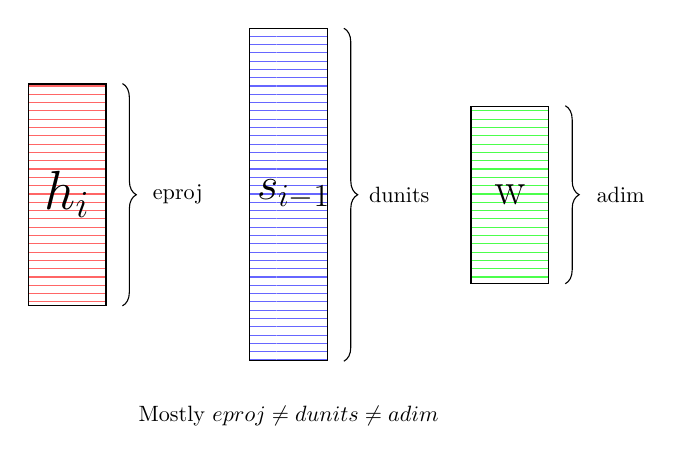
\begin{tikzpicture}[scale=0.8, every node/.style={transform shape}]
			\node [enc_h] (h1) {$h_{i}$};
			\draw [decorate,decoration={brace,amplitude=5pt, mirror, raise=2em}] (h1.south) -- (h1.north) node [black,midway,xshift=5em] {eproj};
			
			\node [dec_z, right of=h1, node distance = 10em, minimum height = 15em] (dec_z) {$s_{i-1}$};
			\draw [decorate,decoration={brace,amplitude=5pt, mirror, raise=2em}] (dec_z.south) -- (dec_z.north) node [black,midway,xshift=5em] {dunits};
			
			\node [atts, right of=dec_z, node distance = 10em, minimum height = 8em] (alpha) {w};
			\draw [decorate,decoration={brace,amplitude=5pt, mirror, raise=2em}] (alpha.south) -- (alpha.north) node [black,midway,xshift=5em] {adim};
			\node [below of=dec_z, node distance = 10em] {Mostly $ eproj \ne dunits \ne adim $};
		\end{tikzpicture}
	\end{center}
	\end{frame}

	\begin{frame}[fragile]{Matching the dimensions of representations}
	\begin{center}
		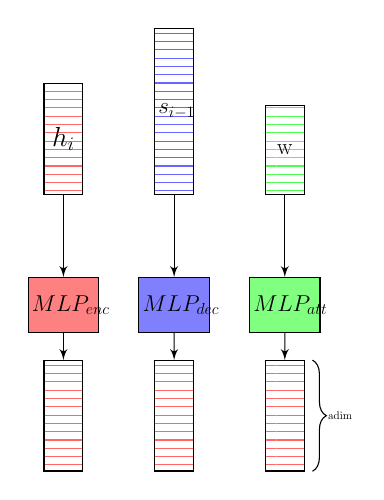
\begin{tikzpicture}[scale=0.4, every node/.style={transform shape}]
			\node [enc_h] (h1) {$h_{i}$};
		
			\node [dec_z, right of=h1, node distance = 10em, minimum height = 15em, yshift=2.5em] (dec_z) {$s_{i-1}$};
			
			\node [atts, right of=dec_z, node distance = 10em, minimum height = 8em, yshift=-3.5em] (alpha) {w};
			
			\node [mlp_enc, below of=h1, node distance = 15em] (mlp_enc) {$MLP_{enc}$};
			\node [mlp_dec, right of=mlp_enc, node distance = 10em] (mlp_dec) {$MLP_{dec}$};
			\node [mlp_att, right of=mlp_dec, node distance = 10em] (mlp_att) {$MLP_{att}$};
			
			\path [line] (h1.south) to (mlp_enc.north);
			\path [line] (dec_z.south) to (mlp_dec.north);
			\path [line] (alpha.south) to (mlp_att.north);
			
			\node [enc_h, below of=mlp_enc, node distance = 10em] (h_att) {};
			\node [enc_h, below of=mlp_dec, node distance = 10em] (z_att) {};
			\node [enc_h, below of=mlp_att, node distance = 10em] (alpha_att) {};
			
			\path [line] (mlp_enc.south) to (h_att.north);
			\path [line] (mlp_dec.south) to (z_att.north);
			\path [line] (mlp_att.south) to (alpha_att.north);
			\draw [decorate,decoration={brace,amplitude=5pt, mirror, raise=1em}] (alpha_att.south) -- (alpha_att.north) node [black,midway,xshift=5em] {adim};
		\end{tikzpicture}
	\end{center}
	\end{frame}


\end{document}
%\begin{frame}[fragile]{title}
%\begin{center}
%	\begin{tikzpicture}[scale=0.3, every node/.style={transform shape}]
%	
%	\end{tikzpicture}
%\end{center}
%\end{frame}